\documentclass[tikz,border=8pt]{standalone}

\usepackage[T1]{fontenc}
\usepackage{lmodern}
\usetikzlibrary{arrows.meta,calc,fit,positioning}

\definecolor{MandateGold}{HTML}{B57A05}
\definecolor{MandateFill}{HTML}{FFF5D9}
\definecolor{TerritorialBlue}{HTML}{1659A5}
\definecolor{TerritorialFill}{HTML}{EEF5FD}
\definecolor{AccessPurple}{HTML}{6C4198}
\definecolor{AccessFill}{HTML}{F5EFFB}
\definecolor{CoordTeal}{HTML}{167A78}
\definecolor{CoordFill}{HTML}{EAF7F5}
\definecolor{SiterBlue}{HTML}{173E78}
\definecolor{Ink}{HTML}{20242A}
\definecolor{Muted}{HTML}{5D6570}
\definecolor{Rule}{HTML}{C8CFD8}
\definecolor{Panel}{HTML}{F8F9FB}

\begin{document}
\sffamily
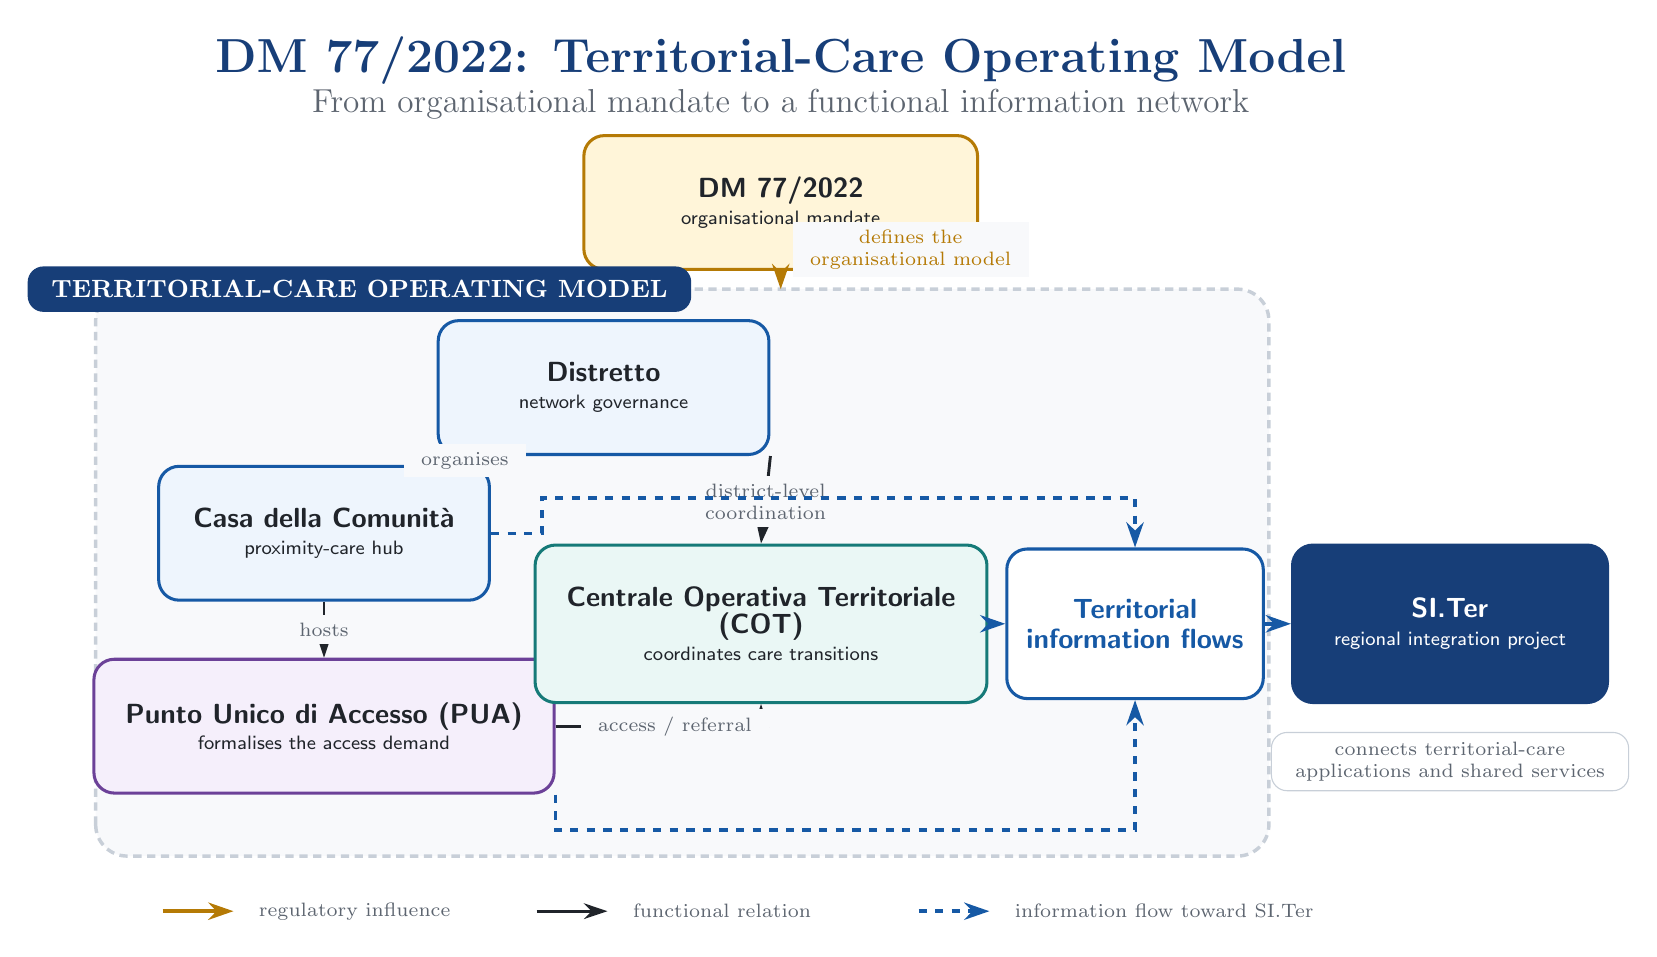
\begin{tikzpicture}[
    font=\sffamily,
    actor/.style={
        rounded corners=2.6mm,
        minimum width=42mm,
        minimum height=17mm,
        inner xsep=4mm,
        inner ysep=3mm,
        align=center,
        line width=1.1pt,
        text=Ink
    },
    relation/.style={-{Stealth[length=3mm,width=2mm]}, line width=1.05pt,
                     draw=Ink},
    info/.style={-{Stealth[length=3.2mm,width=2.2mm]}, line width=1.25pt,
                 draw=TerritorialBlue, dashed},
    regulatory/.style={-{Stealth[length=3.2mm,width=2.2mm]}, line width=1.3pt,
                       draw=MandateGold},
    edge label/.style={fill=Panel, inner xsep=2.2mm, inner ysep=1mm,
                      font=\scriptsize, text=Muted, align=center}
]

% Title
\node[font=\bfseries\LARGE, text=SiterBlue] at (9.25,11.15)
    {DM 77/2022: Territorial-Care Operating Model};
\node[font=\large, text=Muted] at (9.25,10.60)
    {From organisational mandate to a functional information network};

% Regulatory source
\node[actor, draw=MandateGold, fill=MandateFill, minimum width=50mm] (dm) at (9.25,9.35)
    {\textbf{DM 77/2022}\\[-0.8mm]{\scriptsize organisational mandate}};

% Territorial-care model boundary
\filldraw[fill=Panel, draw=Rule, densely dashed, line width=1.25pt,
          rounded corners=4mm] (0.55,1.05) rectangle (15.45,8.25);
\node[fill=SiterBlue, text=white, rounded corners=2mm, inner xsep=3mm,
      inner ysep=1.8mm, font=\bfseries\small] at (3.9,8.25)
    {TERRITORIAL-CARE OPERATING MODEL};
\draw[regulatory] (dm.south) -- (9.25,8.25);
\node[edge label, text=MandateGold] at (10.9,8.75)
    {defines the\\organisational model};

% Organisational actors
\node[actor, draw=TerritorialBlue, fill=TerritorialFill] (district) at (7.0,7.0)
    {\textbf{Distretto}\\[-0.8mm]{\scriptsize network governance}};

\node[actor, draw=TerritorialBlue, fill=TerritorialFill] (community) at (3.45,5.15)
    {\textbf{Casa della Comunità}\\[-0.8mm]{\scriptsize proximity-care hub}};

\node[actor, draw=AccessPurple, fill=AccessFill, minimum width=48mm] (pua) at (3.45,2.70)
    {\textbf{Punto Unico di Accesso (PUA)}\\[-0.8mm]
     {\scriptsize formalises the access demand}};

\node[actor, draw=CoordTeal, fill=CoordFill, minimum width=55mm,
      minimum height=20mm] (cot) at (9.0,4.0)
    {\textbf{Centrale Operativa Territoriale}\\[-0.8mm]
     \textbf{(COT)}\\[-0.8mm]
     {\scriptsize coordinates care transitions}};

% Functional relations
\draw[relation] (district.south west) -- node[edge label, pos=0.52] {organises}
    (community.north east);
\draw[relation] (district.south east) -- node[edge label, pos=0.52]
    {district-level\\coordination} (cot.north);
\draw[relation] (community.south) -- node[edge label] {hosts} (pua.north);
\draw[relation] (pua.east) -- node[edge label, pos=0.58] {access / referral}
    (9.0,2.70) -- (cot.south);

% Information-flow collector inside the model boundary
\node[actor, draw=TerritorialBlue, fill=white, text=TerritorialBlue,
      minimum width=26mm, minimum height=19mm, inner xsep=2.5mm] (flows) at (13.75,4.0)
    {\textbf{Territorial}\\[-0.5mm]\textbf{information flows}};
\draw[info] (community.east) -- ++(0.65,0) -- ++(0,0.45) -| (flows.north);
\draw[info] (pua.south east) -- ++(0,-0.45) -| (flows.south);
\draw[info] (cot.east) -- (flows.west);

% SI.Ter integration layer outside the organisational boundary
\node[actor, draw=SiterBlue, fill=SiterBlue, text=white, minimum width=40mm,
      minimum height=20mm] (siter) at (17.75,4.0)
    {\textbf{SI.Ter}\\[-0.6mm]{\scriptsize regional integration project}};
\draw[info, solid, line width=1.6pt] (flows.east) -- (siter.west);
\node[draw=Rule, rounded corners=2mm, inner xsep=3mm, inner ysep=1.2mm,
      font=\scriptsize, text=Muted, align=center] at (17.75,2.25)
    {connects territorial-care\\applications and shared services};

% Legend
\draw[regulatory] (1.4,0.35) -- (2.3,0.35);
\node[anchor=west, font=\scriptsize, text=Muted] at (2.5,0.35)
    {regulatory influence};
\draw[relation] (6.15,0.35) -- (7.05,0.35);
\node[anchor=west, font=\scriptsize, text=Muted] at (7.25,0.35)
    {functional relation};
\draw[info] (11.0,0.35) -- (11.9,0.35);
\node[anchor=west, font=\scriptsize, text=Muted] at (12.1,0.35)
    {information flow toward SI.Ter};

\end{tikzpicture}
\end{document}
